\documentclass[11pt,a4paper]{article}
\usepackage[danish]{babel}
\usepackage{enumitem}
\usepackage{array, tabularx}
\usepackage[table]{xcolor}
\usepackage{colortbl}
\usepackage{unicode-math}
\usepackage{pgfplots}
\usepackage{tikz}
\usepackage{xurl}            
\usepackage[hidelinks]{hyperref}   
\urlstyle{same}
\pgfplotsset{compat=1.18}

\setlist[enumerate,1]{
    label=\mbox{},        % empty (invisible) label
    leftmargin=0pt,       % align exactly with the text
    labelsep=0pt,
    align=left,
    itemsep=1.5\baselineskip % vertical gap between Opgaver
}
\setlist[enumerate,2]{
    label=(\alph*),
    leftmargin=2em,
    labelsep=.6em,
    itemsep=\baselineskip
}

\title{Matematik Aflevering 2.2}
\author{Luis Conradty \& Carl Hofman}


\begin{document}
  \maketitle
  \begin{enumerate} 
    \item{Opgave 1}
      \begin{enumerate}
        \item
          Forskriften betyder at hvis man køber \(0\) plakater, man betaler \(0\). Hvis man køber mere end et, så skal man betale 2000 kr og 8 til hver nyt man køber.\\
          Primærmængden er \(ℕ_0\) fordi man kan kun købe en naturlig mængde af plakater. Sekundærmængden kan også være \(ℕ_0\), fordi alle priser er i fulde kroner.
        \item
          Ved firma B er det næsten det samme, det starter med \(0\) og hvis man køber mere end et, så skal man betale en gebyr på 1000 kr og hver plakat koster 10 kr.
          Hvis man nu køber flere end tusind styks så bliver den billigere, nemlig kun 6 kr og man skal ikke betale en ekstra gebyr.
          Den \(+5000\) kr skulle kommer fra at betale de 1000 plakater man skal har købt før.
          Faktisk passer forskriften ikke til opgaven, den skal være \(11000\) kr, fordi de tusind plakater koster 10000 kr og startgebyren er 1000
        \item
          \ 
          \begin{figure}[!ht]
            \centering
            \begin{minipage}[t]{0.62\textwidth}
              \vspace{0pt}
                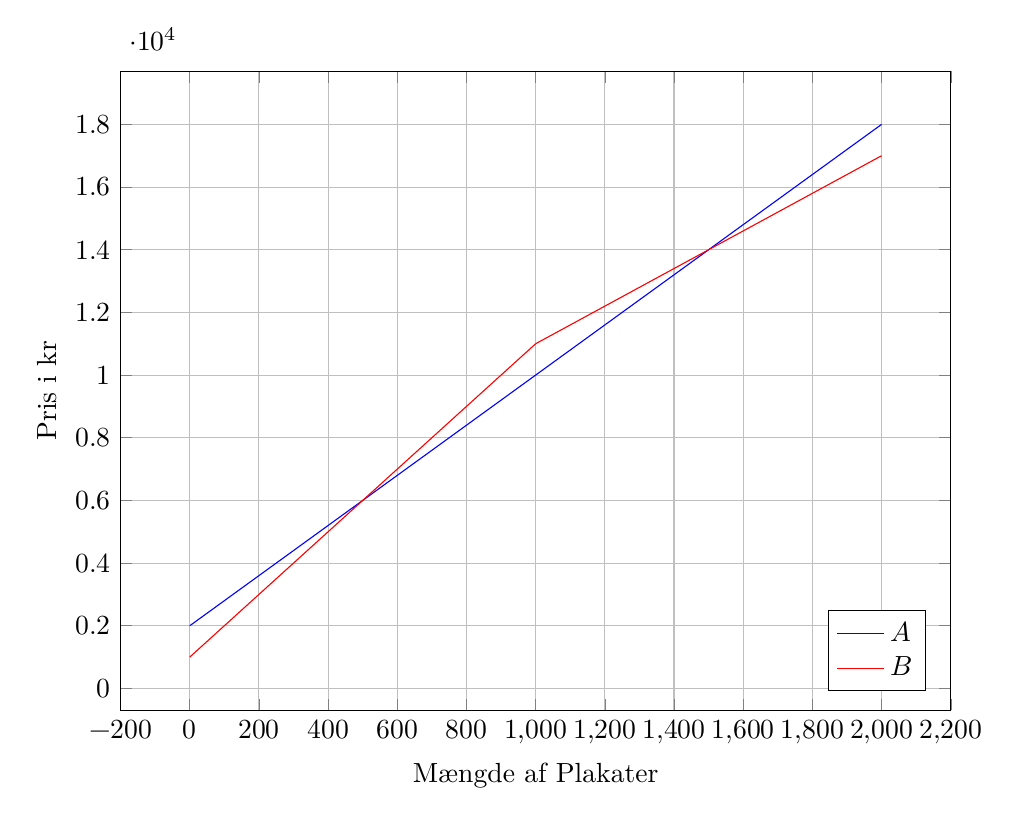
\begin{tikzpicture}
                  \begin{axis}[
                    width=\textwidth,          % fills page text width
                    height=0.8\textwidth,      % pick a pleasing aspect ratio
                    grid=both, xlabel={Mængde af Plakater}, ylabel={Pris i kr}, legend pos=south east
                  ]
                  \addplot+[mark=none, domain=0:2000, samples=400]
                    ({x},{ x<0 ? 0 :  8*x + 2000 });
                  \addlegendentry{\(A\)}
                  \addplot+[mark=none, domain=0:2000, samples=400]
                    ({x},{ x<0 ? 0 : (x<=1000 ? 10*x + 1000  : 6*x + 5000)});
                  \addlegendentry{\(B\)}
                  \end{axis}
                \end{tikzpicture}
            \end{minipage}\hfill
            \begin{minipage}[t]{0.34\textwidth}
              \vspace{0pt}
              \[
                \begin{aligned}
                  A(n) &= \begin{cases}
                    0 &  n=0,\\[2pt]
                    8n+2000 &  n>0
                  \end{cases}\\[6pt]
                  B(n) &= \begin{cases}
                    0 &  n=0,\\[2pt]
                    10n+1000 &  0<n\le 1000,\\[2pt]
                    6n+5000 &  1000<n
                  \end{cases}
                \end{aligned}
              \]
            \end{minipage}
          \end{figure}
        \item
          For at finde hvilken virksomhed er billigere, er det nok at finde hvilken graf er nederst ved hvilken mængder. 
          \begin{align*}
            8n + 2000 &= 10n + 1000 \\
            1000 &= 2n \\
            n &=500
          \end{align*}
          \begin{align*}
            8n + 2000 &= 6n + 5000 \\
            2n &= 3000 \\
            n &= 1500
          \end{align*}

          Det er billigst når man køber ved \(A\) indtil 500 styks og fra 1500 styks. \(B\) er billigere mellem 500 og 1500.

      \end{enumerate}

    \item{Opgave 2}
      \begin{enumerate}
        \item
          Grundmængden for en længde skal være positiv, men der er ingen regler for hvilke slaks positive tal det skal være dermed er grundmængden:
          \[a, b, x, y \in ℝ^+.\]
          \[0\le x < a\]
          \[0\le y < h\]
        \item
          Vi betegner trekantens hjørner med A, B, og C (A er spidsen, med uren). Rektanklens hjørner betegnes med D, E, F, G, starter med den på \(\overline{CA}\) 
          og går også videre med uren.\\
        \(ΔABC\) og \(ΔAED\) er ensvinklet. Det betyder også at forhold mellem sidelængder og højden er det samme. Formlen følges straks:
        \[\frac{h-y}{h} = \frac{\overline{ED}}{\overline{CB}} = \frac{x}{a}\]
          
        \item
          Der kan tegnes en vertikale linje ud fra spidsen af trekanten med et retvinkel mod grundlinjen. Den har længden \(h\) og skærer grundlinjen ved H. 
          Man kan nu brug den samme sætning om ensvinkle trekantes som før, denne gang bare med trekanter \(ΔEBF\) og \(ΔABH\):

          \begin{align*}
            \frac { y } { h } &= \frac { ( a - x ) \cdot \frac { 1 } { 2 } } { a \cdot \frac { 1 } { 2 } } = \frac { a - x } { a } \\
            \Rightarrow y &= \frac { h a - h x } { a } = h - \frac { h } { a } x\\ 
            R ( x ) = x \cdot y &= x \cdot ( h - \frac { h } { a } x ) = h x - \frac { h } { a } x ^ { 2 }\\
          \end{align*}
        \item
          Højdepunktet af parablen eller den største \(x\) findes med formlen: 
          \[x = \frac{-b}{2a} = \frac{-h}{2\frac{h}{a}} = \frac a 2 = 6\]
          Arealet findes ved hjælp af formlen i opgave 2b:
          \[R ( x ) = 16 x - \frac { 16 } { 12 } x ^ { 2 } = 48\]

          Dermed kan y findes:
          \[y = \frac {48} 6 = 8\]

    
    \end{enumerate}
  \item{Opgave 3}
    \begin{enumerate}
      \item
        Dette polynomie er af fjerde grad da det følger forskriften for et fjerdegradspolynomie og at den højeste eksponent er $4$: \[P(x)=x⁴+x³-7x²-x+6\]
      \item
        Man kan bare indsætte røderne og hvis den giver 0, så skal coefficienter også passe.
        \begin{align*}
          P(1) &= 1⁴+ 1³-7\cdot1²- 1+6\\
               &= 1+1-7-1+6\\
               &= 0
        \end{align*}

        \begin{align*}
          P(2) &= 2⁴ + 2³ - 7·2² -2 +6\\
               &= 16 + 8 - 28 - 2 + 6\\
               &= 0
        \end{align*}

      \item
        \ 
        \(P\) har to resterende rødder, nemlig -3 og -1, som kan ses på plottet, disse kan også bevises ved at indsætte dem som x i ligningen:
        \begin{align*}
          P(-3) &= (-3)⁴ + (-3)³ - 7·(-3)² -(-3) +6\\
               &= 81 -27 - 63 +3 + 6\\
               &= 0
        \end{align*}
        \begin{align*}
          P(-1) &= (-1)⁴ + (-1)³ - 7·(-1)² -(-1) +6\\
               &= 1 -1 - 7 +1 + 6\\
               &= 0
        \end{align*}
          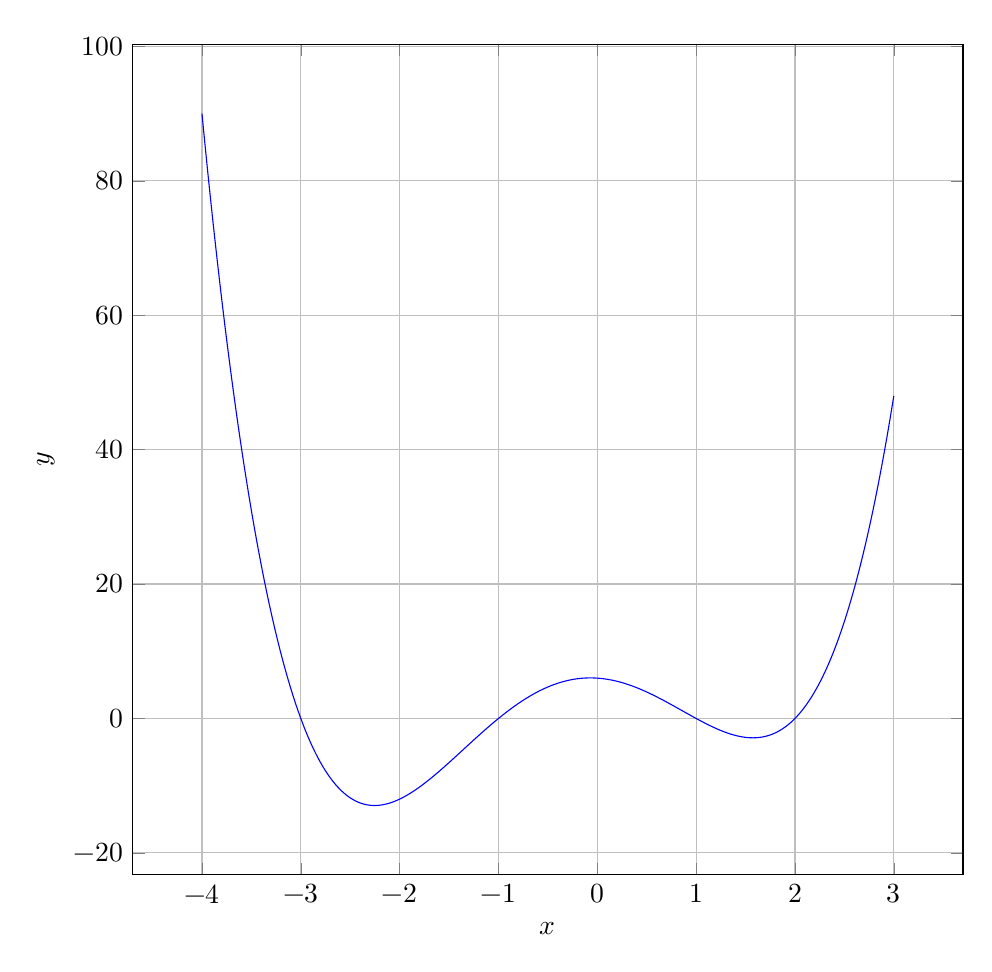
\begin{tikzpicture}
            \begin{axis}[
              width=\textwidth,
              height=\textwidth,
              grid=both, xlabel={$x$}, ylabel={$y$}
            ]
              \addplot+[mark=none, domain=-4:3, samples=400]
                {x^4 + x^3 - 7*x^2 - x + 6};
            \end{axis}
          \end{tikzpicture}
    \end{enumerate}
  \end{enumerate}
\end{document}

